\documentclass[a4paper,12pt]{article}
\pagestyle{empty} % нумерация выкл.
%%% Работа с русским языком
\usepackage{cmap}					% поиск в PDF
\usepackage{mathtext} 				% русские буквы в формулах
\usepackage[T2A]{fontenc}			% кодировка
\usepackage[utf8]{inputenc}			% кодировка исходного текста
\usepackage[english,russian]{babel}	% локализация и переносы
\usepackage{xcolor}
\usepackage{hyperref}
 % Цвета для гиперссылок
\definecolor{linkcolor}{HTML}{799B03} % цвет ссылок
\definecolor{urlcolor}{HTML}{799B03} % цвет гиперссылок

\hypersetup{pdfstartview=FitH,  linkcolor=linkcolor,urlcolor=urlcolor, colorlinks=true}

%%% Дополнительная работа с математикой
\usepackage{amsfonts,amssymb,amsthm,mathtools} % AMS
\usepackage{amsmath}
\usepackage{icomma} % "Умная" запятая: $0,2$ --- число, $0, 2$ --- перечисление

%% Номера формул
%\mathtoolsset{showonlyrefs=true} % Показывать номера только у тех формул, на которые есть \eqref{} в тексте.

%% Шрифты
\usepackage{euscript}	 % Шрифт Евклид
\usepackage{mathrsfs} % Красивый матшрифт

%% Свои команды
\DeclareMathOperator{\sgn}{\mathop{sgn}}

%% Перенос знаков в формулах (по Львовскому)
\newcommand*{\hm}[1]{#1\nobreak\discretionary{}
{\hbox{$\mathsurround=0pt #1$}}{}}
% графика
\usepackage{float}%"Плавающие" картинки
\usepackage{wrapfig}%Обтекание фигур (таблиц, картинок и прочего)
\usepackage{graphicx}
\graphicspath{{pictures/}}
\DeclareGraphicsExtensions{.pdf,.png,.jpg}
\author{Бурмашев Григорий, БПМИ-208}
\title{Матан, дз - 3}
\date{\today}
\begin{document}
\maketitle
\section*{Номер 1}
\[
\sum_{n = 1}^{\infty} \frac{\ln^2n \cos 3n}{\sqrt{2n + 1}}
\]
Попробуем решить по признаку Дирихле:
\begin{center}
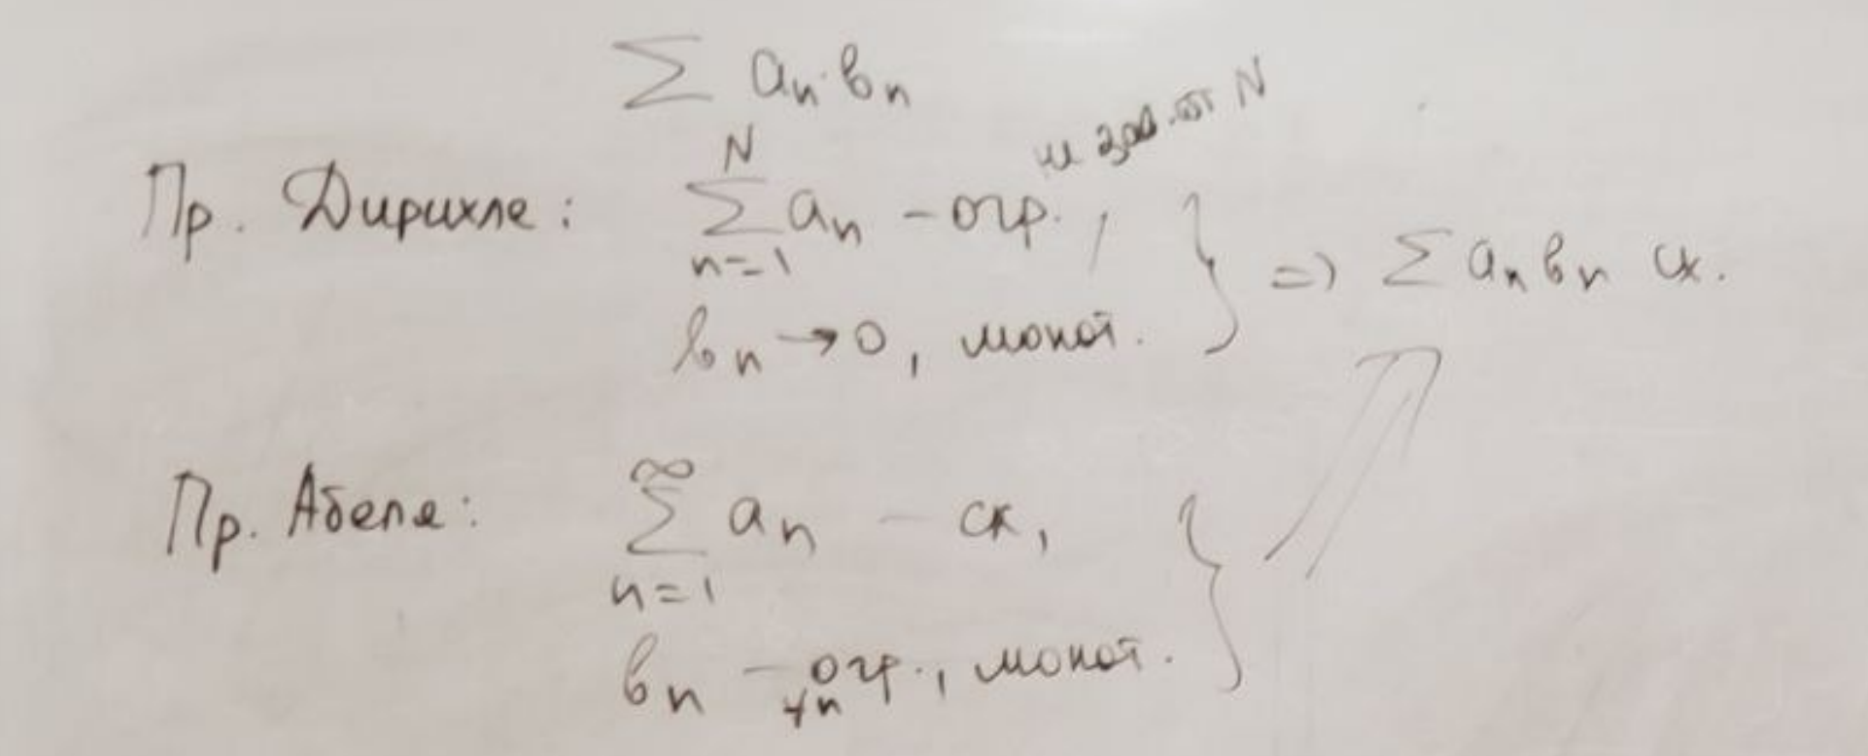
\includegraphics[scale=0.4]{1.png}
\end{center}
Введем обозначения:
\[
a_n = \cos 3n
\]
\[
b_n = \frac{\ln^2 n}{ \sqrt{2n + 1}}
\]
\clearpage
\begin{center}
Начнем проверять условия для Дирихле:
\end{center}
\begin{itemize}
\item На семинаре уже доказали нужное нам, поэтому я думаю бессмысленно перетехивать тоже самое, просто вставлю фотки:
\begin{figure}[h]
\centering
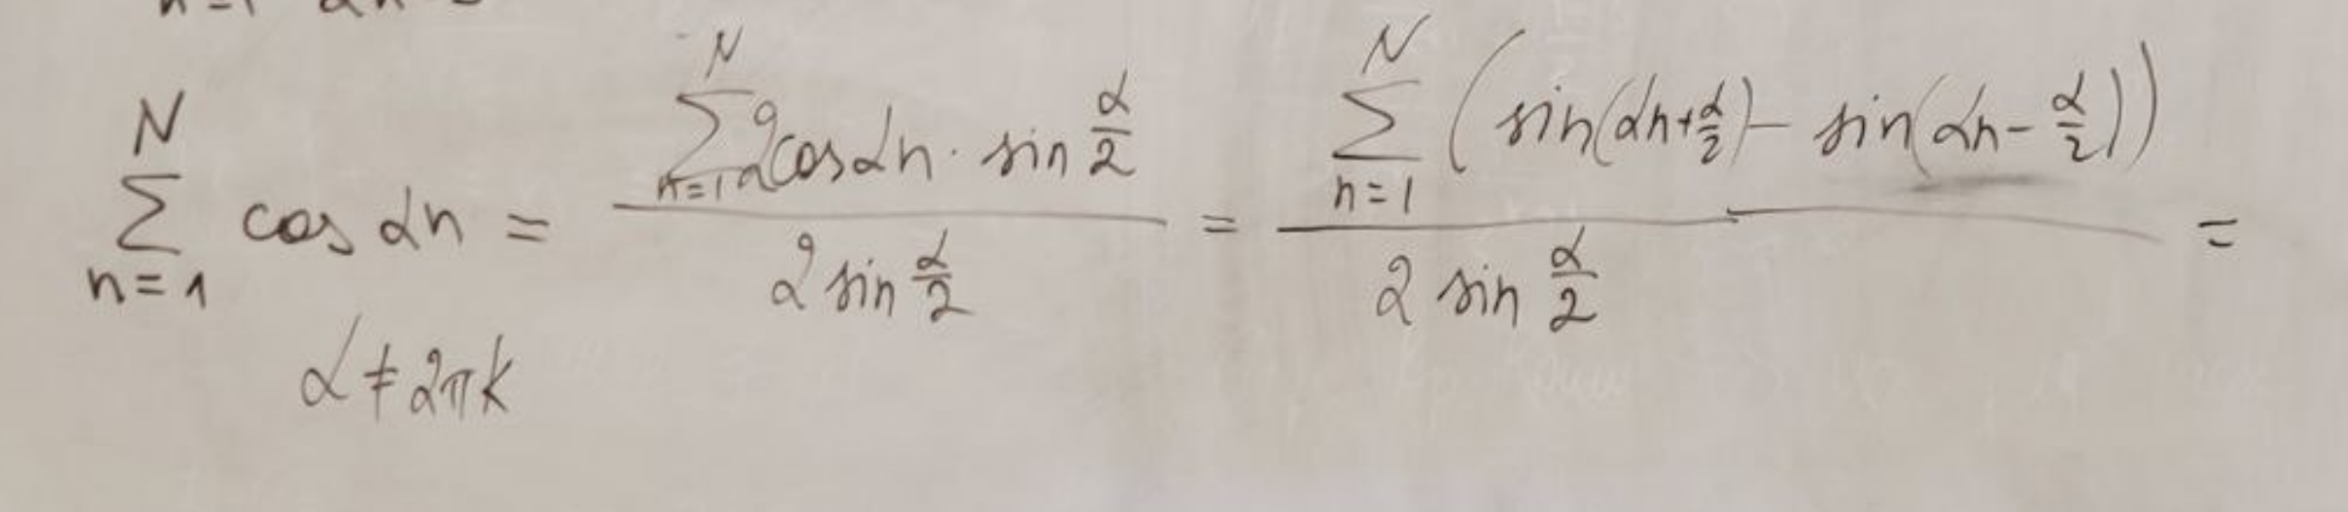
\includegraphics[scale=0.4]{2.png}
\end{figure}
\begin{figure}[h]
\centering
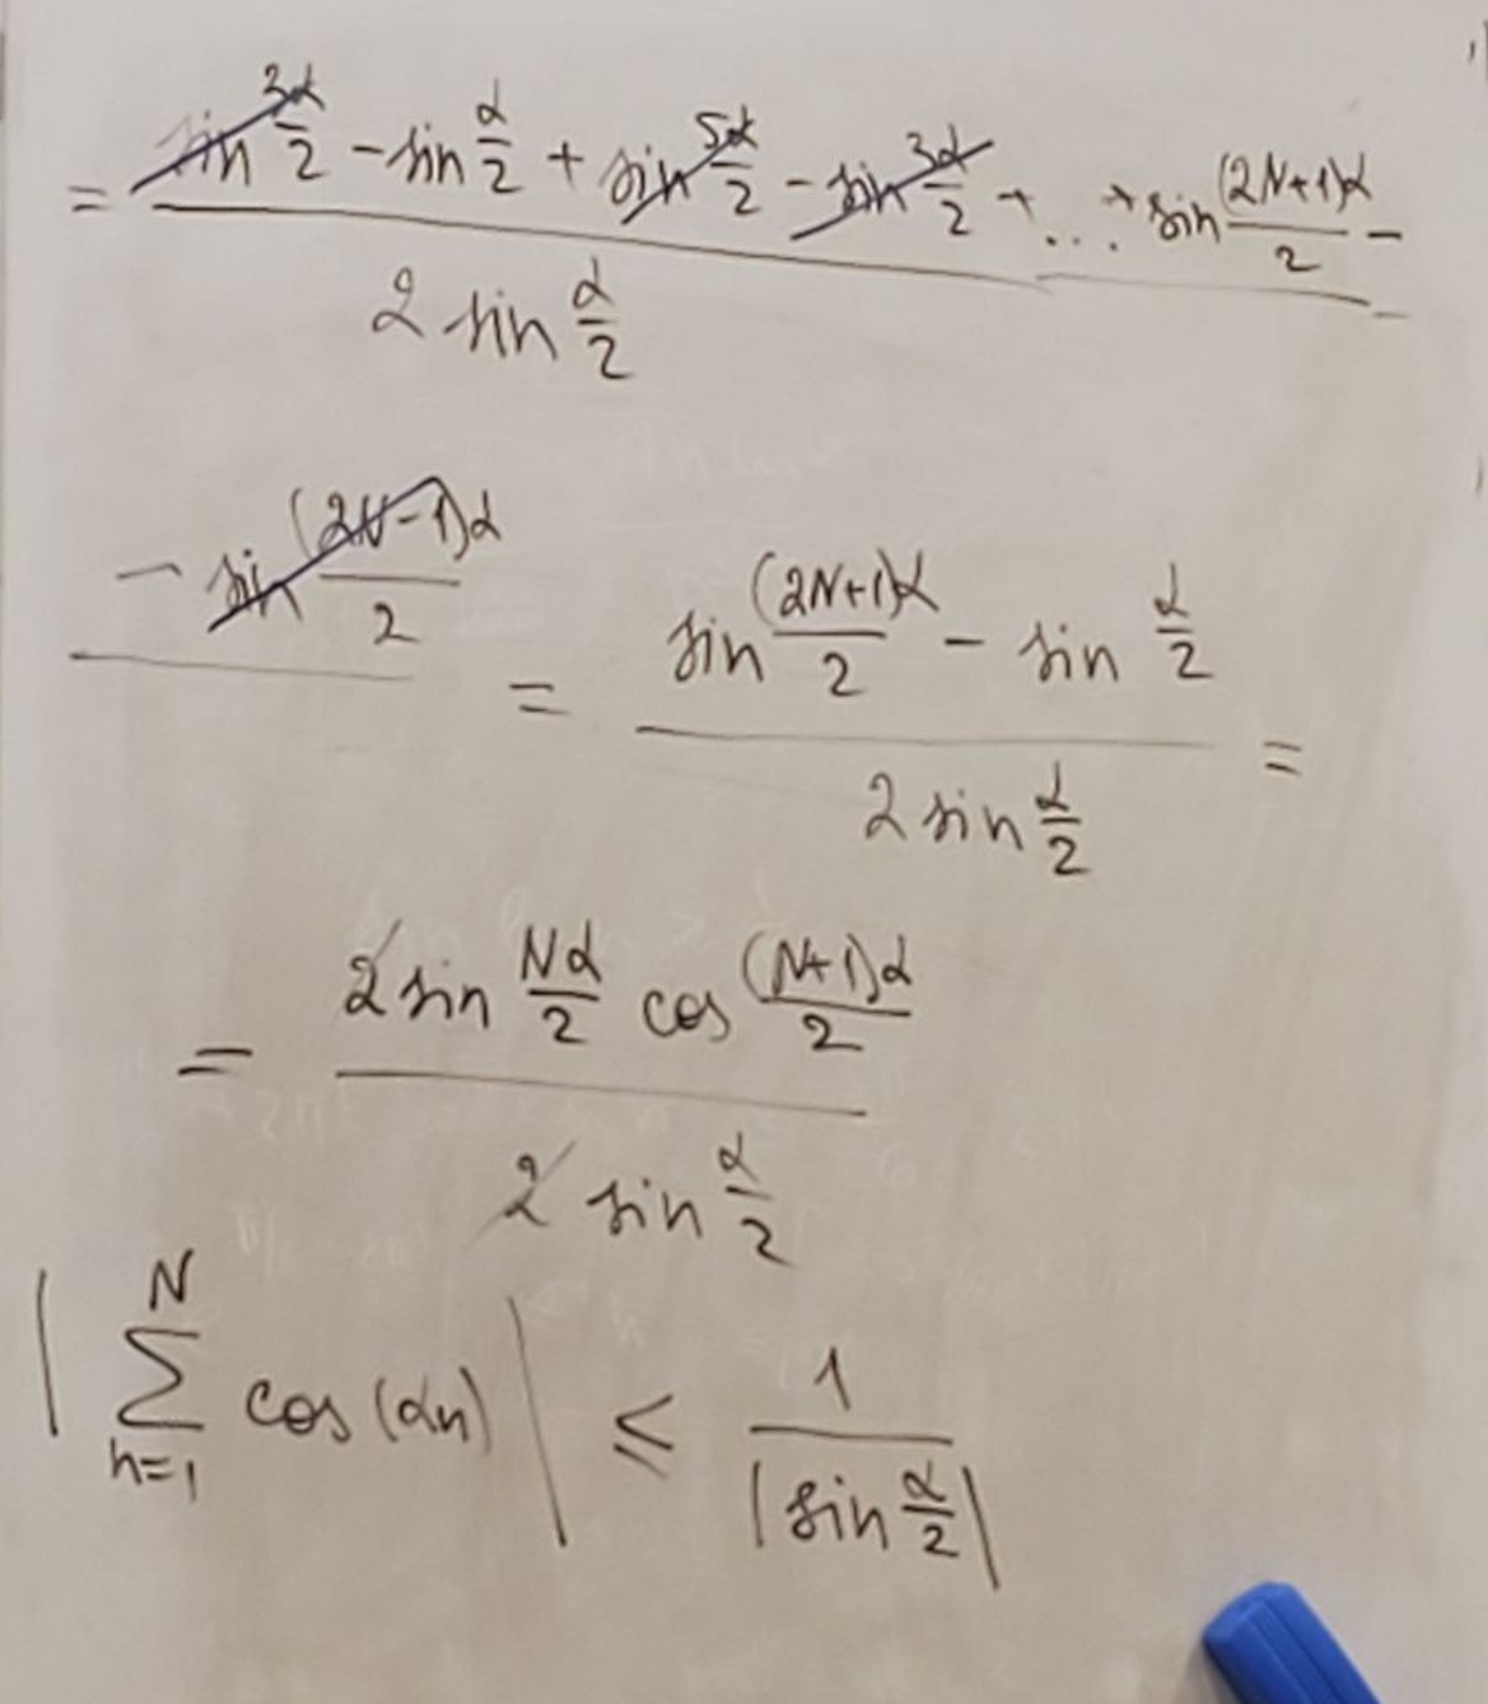
\includegraphics[scale=0.3]{3.png}
\end{figure}
\end{itemize}
\begin{center}
$\rightarrow \sum\limits_{n = 1}^{N} \cos 3n $ ограничен 
\end{center}
\clearpage
\begin{itemize}
\item Проверяем стремление к нулю:
\[
\lim_{n \rightarrow \infty }\frac{\ln^2 n}{ \sqrt{2n + 1}} = \left[ \frac{\infty}{\infty} \right] = \lim_{n \rightarrow \infty } \frac{\frac{2\ln n}{n}}{\frac{1}{\sqrt{2n + 1}}} = \lim_{n \rightarrow \infty } \frac{2 \ln n \cdot \sqrt{2n + 1}}{n} = 
\]
\[
= \lim_{n \rightarrow \infty } \frac{4n +2 n \ln n + 2}{n \sqrt{2n + 1}} = \lim_{n \rightarrow \infty } \left( \frac{4}{ \sqrt{2n + 1}} + \frac{2 \ln n}{\sqrt{2n + 1}}+ \frac{2}{n \sqrt{2n + 1}}  \right) = 
\]
\[
 \lim_{n \rightarrow \infty } \left( \frac{4}{ \sqrt{2n + 1}} \right) +\lim_{n \rightarrow \infty } \left( \frac{2 \ln n}{\sqrt{2n + 1}} \right)+\lim_{n \rightarrow \infty } \left( \frac{2}{n \sqrt{2n + 1}}  \right) =
\] 
\[
= 0 + 0  \text{ (т.к ln медленее корня}) + 0  = 0
\]
\begin{center}
\textbf{Выполняется}
\end{center}
\item Проверяем монотонность, для этого возьмем производную:
\[
\left( \frac{\ln^2n}{\sqrt{2n + 1}} \right)' = \frac{\frac{2 \ln n}{n } \cdot \sqrt{2n + 1} - \ln^2 n \cdot \frac{1}{\sqrt{2n+1}}}{2n + 1} = \frac{\frac{2 \ln n \cdot \sqrt{2n + 1}}{n} - \frac{\ln^2 n }{\sqrt{2n + 1}}}{2n + 1} = 
\]
\[
= \frac{\frac{2\ln n \cdot (2n + 1) - ln^2 n \cdot n}{n \cdot \sqrt{2n + 1}}}{2n + 1} = \frac{2\ln n \cdot  (2n + 1) - \ln^2 n \cdot n}{(2n+1) \cdot n \cdot \sqrt{2n + 1}} = \frac{\ln n (4n + 2- \ln n \cdot n)}{(2n+1) \cdot n \cdot \sqrt{2n + 1}}
\]
Теперь заметим, что:
\[
(2n + 1) \cdot n \cdot \sqrt{2n + 1} > 0 
\]
\[
\ln n \geq 0 
\]
\[
4n + 2 - \ln n \cdot n < 0, \text{ т.к } \ln n \cdot n > 4n + 2 \text{ начиная с некоторого } n_i
\]
 А значит все выражение $\leq 0$,  т.е:
\[
(b_n)' \leq 0 \rightarrow b_n \text{ монотонно убывает }
\]
\begin{center}
\textbf{Выполняется}
\end{center}
\end{itemize}
Все необходимые для признака Дирихле условия выполняются, а значит ряд \textbf{сходится}
\begin{center}
\textbf{Ч.Т.Д} 
\end{center}










\clearpage
\section*{Номер 2}
\[
\sum_{n=1}^{\infty}\frac{(-1)^{\left[\sqrt[3]{n}\right]}}{\sqrt[3]{n^2 + 3}}
\] 
Решаю аналогично подобным задачам с семинара, избавимся от $\left[\right]$ путем замены, получим новый ряд и посмотрим сходится ли абсолютно. 
\\\\
Пусть $\left[\sqrt[3]{n}\right] = k$, тогда:
\[
k \leq \sqrt[3]{n} < k + 1 
\]
\[
k^3 \leq n < (k + 1)^3
\]
\[
\left[k^3\right] + 1 \leq n \leq \left[(k + 1) ^3 \right]
\]
Теперь смотрим на новый ряд:
\[
\Bigg|
\sum_{n = \left[k^3\right] + 1}^{\left[(k+1)^3\right]} \frac{(-1)^k}{\sqrt[3]{n^2 + 3}} \Bigg| = \sum_{n = \left[k^3\right] + 1}^{\left[(k+1)^3\right]} \frac{1}{\sqrt[3]{n^2 + 3}} \geq  \frac{\left[(k+1)^3\right] - \left[k^3\right]}{\sqrt[3]{(\left[(k+1)^3\right])^2 + 3}} \geq \frac{(k+1)^3 - 1 - k^3}{\sqrt[3]{(k+1)^6 + 3}} \geq \]

\[
\geq \frac{k^3 + 3k^2 + 3k + 1 -1  -k^3 }{\sqrt[3]{(k + 1)^6 + 3}} \geq \frac{3k^2 + 3k}{\sqrt[3]{(k + 1)^6 + 3}} =
\]
Не очень хочется раскрывать многочлен 6й степени, поэтому можно просто заметить очевидный факт, что он будет вида $k^6 + bk^5 + \ldots$, поэтому при делении на $k^2$ (под корнем 3й степени это будет $k^6$ соотв.) все множители, кроме первого, при $k \rightarrow \infty$ уйдут в ноль, а первый множитель будет $\frac{k^6}{k^6} = 1$, поэтому дробь примет вид:
\[
= \frac{3 + \frac{3}{k}}{\sqrt[3]{1 + \frac{b}{k} + \ldots}} \underset{k \rightarrow \infty}{\longrightarrow} \frac{3}{\sqrt[3]{1}} = 3 \neq 0 
\]
Отр.Кр.Коши $\rightarrow$ исходный ряд расходится
\begin{center}
\textbf{Ч.Т.Д } 
\end{center}
\end{document}
